\documentclass[a4paper]{article}
\usepackage[top=2cm, bottom=2cm, left=2cm, right=2cm]{geometry}

\usepackage[T1]{fontenc}
\usepackage[utf8]{inputenc}

\usepackage{graphicx}          % To handle figures
\usepackage{amsmath}           % Defines certain mathematical symbols
\usepackage{amsfonts}
\usepackage{pdfpages}

\renewcommand{\thesubsection}{\arabic{section}.\alph{subsection}}

\begin{document}


%---------------------------------------------------------------------------------------------------------
%Title
\newcommand{\HRule}{\rule{\linewidth}{0.5mm}} 
\title{{\LARGE EQ2410 - Advanced Digital Communications} \\[0.5cm] \HRule \\[0.4cm]{Project 1 : Channel Equalization}\\[0.2cm] \HRule \\[0.5cm] }
\author{Baptiste Cavarec \\ 940321-T197 \and Hugo Lime\\  920707-4635 \and Adrien Anxionnat\\ \#\#\#\#\#\#-\#\#\#\#}
%\date{2000-10-10}

\maketitle



%---------------------------------------------------------------------------------------------------------
%Problem 1
\section{Problem 1}
\subsection{Identification of signals}
\begin{itemize}
  	\item \verb|Vect_1|: Random QPSK data symbol sequence\\ 
  $	\verb|Vect_1| \in {\{1+i, 1-i, -1+i, -1-i\}}^{\verb|N_symbols|} $
  	\item \verb|Signal_1|: \verb|Vect_1| upsampled by factor \verb|T_sym|/ \verb|delta_t| and normalized\\
  	$\verb|Signal_1|(1+k*\verb|T_sym|/ \verb|delta_t|)=\verb|Vect_1|(1+k)/ \verb|delta_t|$ with $k\in [0, \verb|N_symbols|-1]$
  	\item \verb|Signal_2|: Complex baseband data transmitted waveform\\
  	$\verb|Signal_2|=\verb|Signal_1|\star \verb|Filter_1|$
  	\item \verb|Signal_3|: Complex baseband data received waveform\\
  	$\verb|Signal_3|=\verb|Signal_2|\star \verb|Filter_2|$
  	\item \verb|Signal_4|: Complex baseband noise waveform with two-sided variance $N_0$ 
  	\item \verb|Signal_5|: Complex baseband total received waveform\\
  	$\verb|Signal_5|=\verb|Signal_3| + \verb|Signal_4|$
  	\item \verb|Signal_6|: Complex baseband total received waveform matched filtered\\
  	$\verb|Signal_6|=\verb|Signal_5|\star \verb|Filter_4|$
  	\item \verb|Vect_2|: Sampler output received symbol sequence after synchronization\\
  	$\verb|Vect_2|(k)= \verb|Signal_6|(k*\verb|T_sample|/ \verb|delta_t|+\delta_{offset})$ (\verb|Signal_6| downsampled)
\end{itemize}

\subsection{Identification of filters}
\begin{itemize}
	\item \verb|Filter_1|: Transmitter filter
	\item \verb|Filter_2|: Channel filter
	\item \verb|Filter_3|: Transmitter and Channel chain filter
	\item \verb|Filter_4|: Matched filter of \verb|Filter_3|, can be used as receiver filter
	\item \verb|Filter_5|: Transmitter, channel and receiver chain filter, used to simulate the overall system response
\end{itemize}

\subsection{Normalization coefficient}
In the program, we use a small time resolution (\verb|delta_t|) to represent continuous-time signals. We consider the signals to be constant over these small intervals. With this approximation, the integrals, used in the convolutions for example, are transformed into sums in the following way:
\begin{equation*}
(f\star g)(m\delta_{t}) = \int_{-\infty}^{+\infty} f(t)g(m\delta_{t}-t) dt = \sum_{k=-\infty}^{\infty}\left(\int_{k\delta_{t}}^{(k+1)\delta_{t}} f(t)g(m\delta_{t}-t) dt \right) \approx \delta_{t}\sum_{k=-\infty}^{\infty}f(k\delta_{t})g((m-k)\delta_{t})
\end{equation*}

And we can notice that, compared to the discrete-time convolution formula used by Matlab, the last sum is multiplied by \verb|delta_t|.\\

The factor $1/\verb|delta_t|$ when we generate \verb|Signal_1| is another normalization used to keep the signal power indepedant of the time resolution. In the same manner we have:
\begin{align*}
P &=\frac{1}{N_{symbols}T_{sym}}\int_{0}^{N_{symbols}T_{sym}}|S_{1}(t)|^{2}dt\\
&\approx \frac{1}{N_{symbols}T_{sym}}\sum_{k=0}^{(N_{symbols}-1)T_{sym}\delta_t}|S_{1}(k\delta_t)|^{2}\delta_t\\ &\approx\frac{{\delta_t}^2}{N_{symbols}T_{sym}\delta_t}\sum_{k=0}^{(N_{symbols}-1)T_{sym}\delta_t}|S_{1}(k\delta_t)|^{2}\\
&\approx\frac{1}{N_{symbols}T_{sym}\delta_t}\sum_{k=0}^{(N_{symbols}-1)T_{sym}\delta_t}|\delta_t^2S_{1}(k\delta_t)|^{2} 
\end{align*}
And by dividing by $1/\verb|delta_t|$, the discrete-time signal power of \verb|Signal_1| is independant of \verb|delta_t| and equal to the one of \verb|Vect_1|.

%---------------------------------------------------------------------------------------------------------
%Problem 2
\section{Problem 2}
We know that $\mathbf{r}[n]=\mathbf{Ub}[n]+\mathbf{w}[n]$, that $\mathbf{R}=\mathbb{E}[\mathbf{r}[n]{\mathbf{r}[n]}^H]$ and that $\mathbf{p}=\mathbb{E}[b^*[n]\mathbf{r}[n]]$\\
Therefore:
\begin{equation*}
\mathbf{r}[n]^H=\mathbf{b}[n]^H\mathbf{U}^H+\mathbf{w}[n]^H\\
\end{equation*}
so that:
\begin{equation}
\label{rr}
\mathbf{r}[n]\mathbf{r}[n]^H = \mathbf{U}\mathbf{b}[n]\mathbf{b}[n]^H\mathbf{U}^H + \mathbf{U}\mathbf{b}[n]\mathbf{w}[n]^H+\mathbf{w}[n]\mathbf{b}[n]^H\mathbf{U}^H+\mathbf{w}[n]\mathbf{w}[n]^H
\end{equation}
with
\begin{equation*}
\mathbb{E}[\mathbf{w}[n]\mathbf{w}[n]^H] = \mathbf{C_w}
\end{equation*}
As the data values $b[n]$ are independant, we have
\begin{equation*}
\mathbb{E}[\mathbf{b}[n]\mathbf{b}[n]^H] = P_s\mathbf{I}\text{\hspace{2cm}with } P_s=\mathbb{E}[|b[n]|^2]
\end{equation*}
Moreover, as $b[n]$ and $w[k]$ are independant for every $n$ and $k$, it remains in the expectation of (\ref{rr}): 
\begin{equation}
\mathbf{R}=P_s\mathbf{U}\mathbf{U}^H + \mathbf{C_w}
\end{equation}\\ 

We can also write:
\begin{equation}
\label{br}
b^*[n]\mathbf{r}[n]=\mathbf{U}b^*[n]\mathbf{b}[n] + b^*[n]\mathbf{w}[n]
\end{equation}
and $b[n]$ is independant of $w[k]$ for every $k$ and independant of $b[k]$ for every $k\ne1$. It gives:
\begin{equation*}
\mathbb{E}[b^*[n]\mathbf{b}[n]]=P_s\mathbf{e}
\end{equation*}

Taking the expectation of (\ref{br}), it remains:
\begin{equation}
\mathbb{E}[b^*[n]\mathbf{r}[n]]=P_s\mathbf{Ue}
\end{equation}

\newpage
%---------------------------------------------------------------------------------------------------------
%Problem 3
\section{Problem 3}

\begin{figure}[ht!]
\centering
\begin{center}
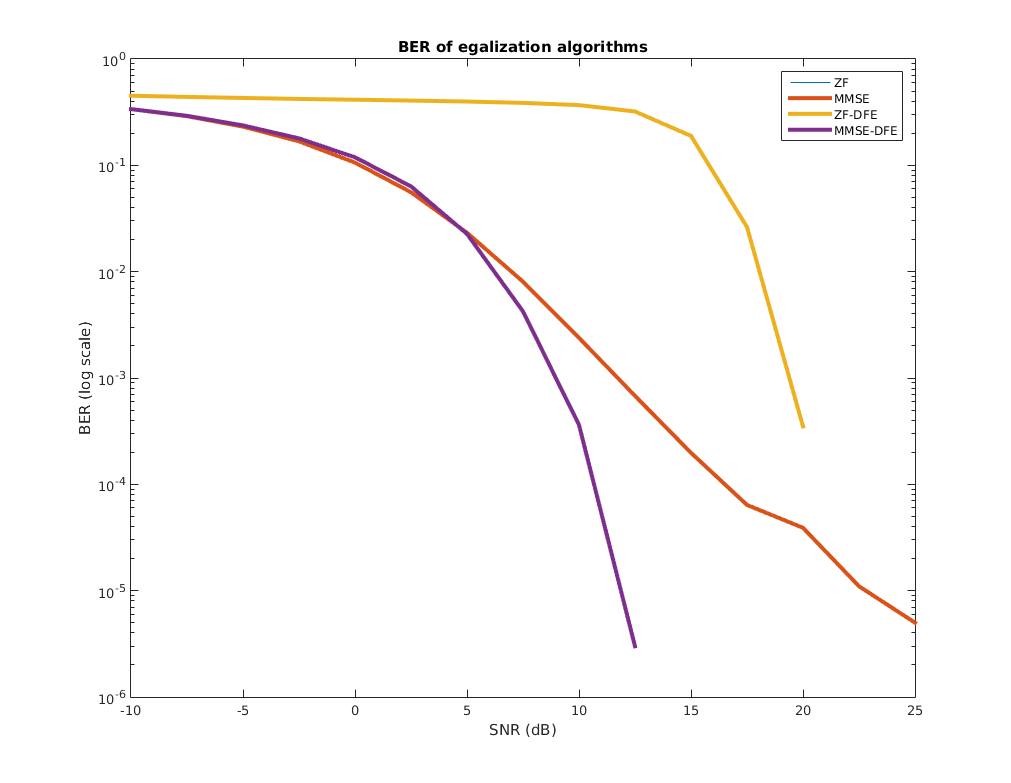
\includegraphics[scale=0.50]{BER-m1.png}
\caption{BER comparison for $m=1$}
\label{m1}
\end{center}
\end{figure}

Figure \ref{m1} confirm the results in Figure 5.14 of Upamanyu Madhow, Fundamentals of Digital Communication.

\begin{figure}[ht!]
\centering
\begin{center}
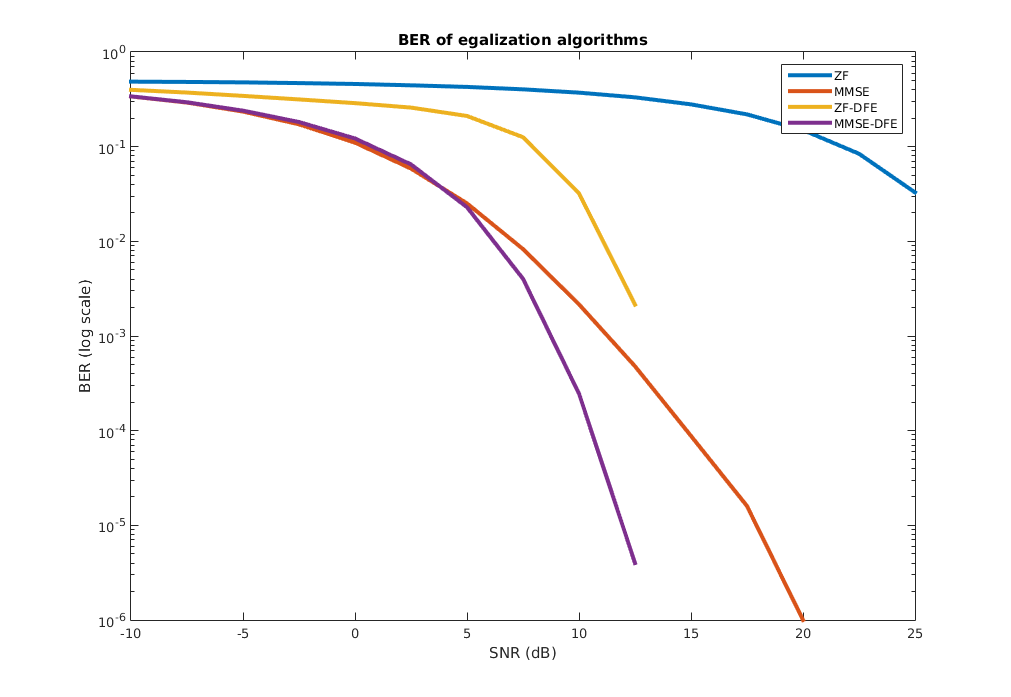
\includegraphics[scale=0.50]{BER-m2.png}
\caption{BER comparison for $m=2$}
\label{m2}
\end{center}
\end{figure}
%---------------------------------------------------------------------------------------------------------
%Problem 4
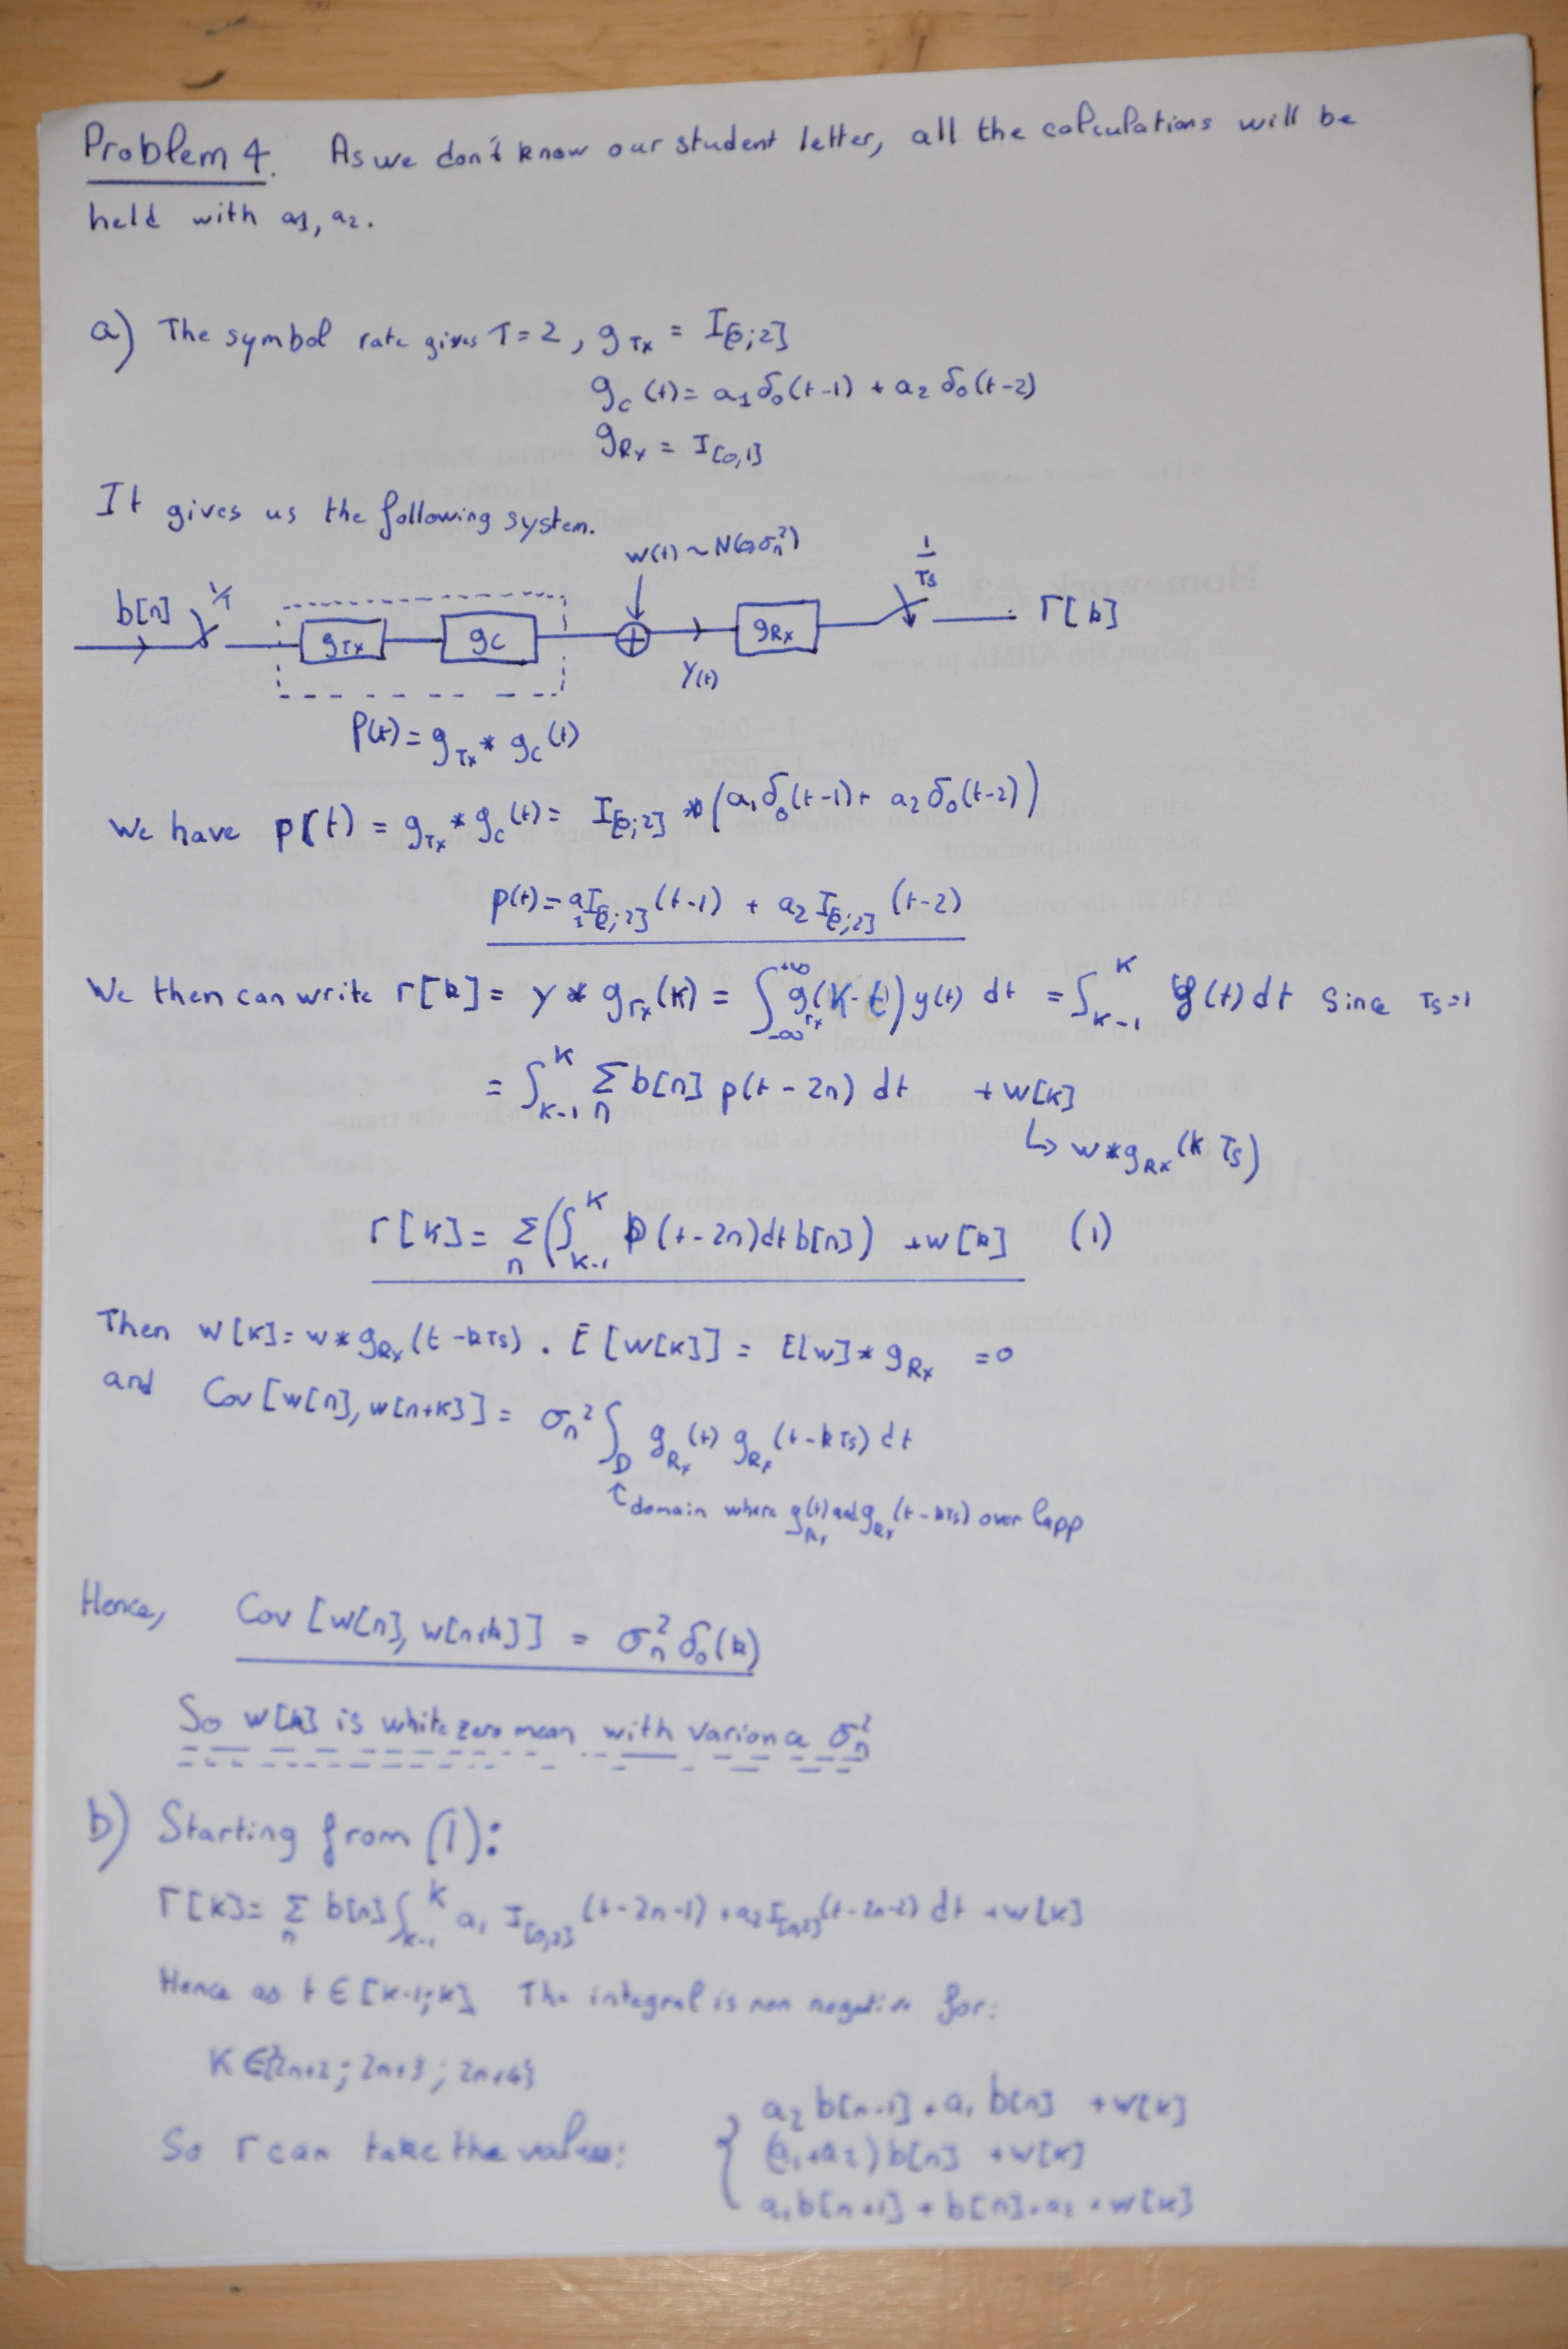
\includepdf[pages={1,2,3,4}]{Problem4SQ.pdf}
%---------------------------------------------------------------------------------------------------------
\end{document}